% !TeX root = ../libro.tex
% !TeX encoding = utf8
%
%*******************************************************
% Series Temporales
%*******************************************************

\chapter{Series Temporales}\label{ch:st}

Presentamos y explicamos la teoría sobre las \textbf{series temporales}, los objetos de estudio que se presentarán en nuestros problemas y que se usarán en los modelos realizados.

Usaremos como base para desarrollar esta parte la literatura para series temporales y procesos estocásticos, concretamente de \cite{cox1977theory}, \cite{chatfield2019analysis}, \cite{brockwell2002introduction}, \cite{hyndman2018forecasting}, \cite{box2011time} y \cite{grandell1998time}.

\section{Definición y características}

Para ver qué es y poder estudiar una serie temporal necesitamos tener una base de la teoría de \textbf{procesos estocásticos}. Esta teoría se encarga de estudiar sistemas que evolucionan en el \textbf{tiempo} en función de \textbf{leyes probabilísticas}.

\subsection{Elementos básicos}

Para explicar estos conceptos vamos a hacer un breve recordatorio de los elementos fundamentales que juegan un papel en la teoría de la probabilidad, que se basa en el estudio de ciertas \textbf{funciones} reales que parten de un espacio donde hay una \textbf{medida de probabilidad}.

La idea del espacio que hemos mencionado es muy simple: queremos asignar a \textbf{subconjuntos} (sucesos) de cierto \textbf{espacio} una cantidad numérica que representa la \textbf{probabilidad} de que ocurran. Por tanto necesitaremos un espacio $\Omega$, una $\sigma$-álgebra $\mathcal{A}$ sobre $\Omega$ (\autoref{def:sigma-algebra}) y una función de probabilidad $P$ en $\Omega$ (\autoref{def:probabilidad}).

\begin{definicion}[$\sigma$-álgebra]
  Sea un conjunto $\Omega$, una $\sigma$-álgebra sobre $\Omega$ es una familia $\mathcal{A}$ de subconjuntos de $\Omega$ que incluye el espacio entero y es cerrada bajo complementos y uniones numerables; es decir, que cumple lo siguiente:
  \begin{enumerate}
    \item $\Omega \in \mathcal{A}$.
    \item $\forall A \in \mathcal{A} \implies \overline{A} \in \mathcal{A}$.
    \item $\forall \{A_n\}_{n \in \N} \subseteq \mathcal{A} \implies \bigcup \limits^\infty_{n = 1} A_n \in \mathcal{A}$
  \end{enumerate}
  \label{def:sigma-algebra}
\end{definicion}

\begin{definicion}[Función de probabilidad]
  Sea un espacio $\Omega$, y $\mathcal{A}$ una $\sigma$-álgebra sobre $\Omega$, una función de probabilidad $P : \mathcal{A} \to R$ es una función que cumple lo siguiente:

  \begin{itemize}
    \item (No negativa): $\forall A \in \mathcal{A}, \, P(A) \geq 0$
    \item (Normalización): $P(\Omega) = 1$
    \item ($\sigma$-aditividad): $\forall \{A\}_{n \in \N} \subseteq \mathcal{A}$ disjuntos 2 a 2 $\implies P \left(\bigcup \limits^\infty_{n = 1} A_n \right) = \sum \limits^\infty_{n = 1} P(A_n)$
  \end{itemize}
  \label{def:probabilidad}
\end{definicion}

Juntando estos tres elementos obtenemos nuestro \textbf{espacio probabilístico} (\autoref{def:espacio-probabilistico}).

\begin{definicion}[Espacio probabilístico]
  Sea $\Omega$ un conjunto, $\mathcal{A}$ una $\sigma$-álgebra sobre $\Omega$ y $P$ una probabilidad en $\Omega$, entonces definimos el espacio de probabilidad como la terna $(\Omega, \mathcal{A}, P)$.
  \label{def:espacio-probabilistico}
\end{definicion}

Como la probabilidad $P$ es realmente una medida normalizada, podemos aplicar aspectos de la teoría de la medida en un espacio probabilístico. En concreto consideraremos funciones medibles, que son aplicaciones medibles (\autoref{def:aplicacion-medible}) donde el espacio de llegada es un espacio \textbf{Borel} ($\sigma$-álgebra formada con las semirectas cerradas por la derecha $(-\infty, x]$).

\begin{definicion}[Aplicación medible]
  Sean dos espacios medibles $(\Omega_1, \mathcal{A}_1)$, $(\Omega_2, \mathcal{A}_2)$, una aplicación $f : \Omega_1 \to \Omega_2$ se dice medible, si y solamente si:

  $$\forall A \in \mathcal{A}_2, \, f^{-1}(A) = \{\omega \in \Omega_1 : f(\omega) \in A\} \in \mathcal{A}_1$$
  \label{def:aplicacion-medible}
\end{definicion}

Definimos así las funciones que forman la base de esta teoría: las \textbf{variables aleatorias} (\autoref{def:var-aleatoria}). Hemos tomado el espacio Borel usual como $(\R, \mathcal{B})$ aunque si tenemos un subconjunto $E \subseteq \R$ se puede considerar el espacio Borel $(E, \mathcal{B}_E)$ donde $\mathcal{B}_E$ es la $\sigma$-álgebra Borel restringida a $E$.

\begin{definicion}[Variable aleatoria]
  Sea un espacio de probabilidad $(\Omega, \mathcal{A}, P)$, una variable aleatoria es una función medible de un espacio de probabilidad en un espacio Borel $X: (\Omega, \mathcal{A}, P) \to (\R, \mathcal{B})$.
  \label{def:var-aleatoria}
\end{definicion}

Una variable aleatoria $X$ induce una probabilidad en el espacio de llegada Borel que denominamos como \textbf{función de probabilidad} (\autoref{def:distribucion-probabilidad}).

\begin{definicion}[Distribución de probabilidad]
  Sea un espacio probabilístico $(\Omega, \mathcal{A}, P)$ y una variable aleatoria $X: (\Omega, \mathcal{A}, P) \to (\R, \mathcal{B})$, llamamos distribución de probabilidad de una variable aleatoria a una función de probabilidad definida en el espacio Borel, dada por:

  $$\begin{aligned} P_X : \mathcal{B} & \to \R \\
      B & \mapsto P_X(B) = P(X^{-1}(B)) = P[X \in B]
    \end{aligned}.$$
  \label{def:distribucion-probabilidad}
\end{definicion}

Si recordamos, la $\sigma$-álgebra Borel $\mathcal{B}$ estaba generada por las semirrectas abiertas por la derecha ($(-\infty, x]$), por lo que podemos definir la distribución como una función de variable real: \textbf{ffunción de distribución} (\autoref{def:funcion-distribucion}).

\begin{definicion}[Función de distribución]
  Sea un espacio probabilístico $(\Omega, \mathcal{A}, P)$ y una variable aleatoria $X: (\Omega, \mathcal{A}, P) \to (\R, \mathcal{B})$, Llamamos función de distribución a la función definida de la siguiente forma:

  $$\begin{aligned} F_X : \R & \to \R \\
      x & \mapsto F_X(x) = P_X((-\infty, x]) = P[X \leq x]
    \end{aligned}.$$
\label{def:funcion-distribucion}
\end{definicion}

Cabe añadir que todo lo que hemos visto de teoría es fácilmente extensible al caso multidimensional (cuando el espacio Borel es multidimensional $R^n$) ya que se considera $X = (X_1, \ldots, X_n)$ como un \textbf{vector aleatorio} donde $X_i$ es una variable aleatoria $i = 1, \ldots, n$.

\subsection{Procesos estocásticos}

Ya podemos definir qué es un \textbf{proceso estocástico}, que no es más que una sucesión de variables aleatorias ordenadas por el tiempo (\autoref{def:proceso-estocastico}).

\begin{definicion}[Proceso estocástico]
  Sea un espacio de probabilidad $(\Omega, \mathcal{A}, P)$, un conjunto ordenado arbitrario $T$, un espacio Borel $(E, \mathcal{B}_E)$ y las variables aleatorias $X_t : (\Omega, \mathcal{A}, P) \to (\R, \mathcal{B}), \, \forall t \in T$. Un proceso estocástico es una familia de variables aleatorias $\{X_t\}_{t \in T}$ ordenadas por $T$.
  \label{def:proceso-estocastico}
\end{definicion}

Notamos $T$ como el \textbf{espacio paramétrico} y es a lo que nos referimos como el tiempo. Según quién sea $T$ podemos decir que el proceso es en \textbf{tiempo discreto} ($T = \N \cup \{0\}$) o en \textbf{tiempo continuo} ($T = [0, + \infty)$). Además, el espacio Borel de llegada se denomina como \textbf{espacio de estados} y nos permite clasificar el proceso como \textbf{discreto} (si $E$ es discreto) o \textbf{continuo} (si $E$ es no numerable).

Listamos unos cuantos ejemplos ilustrativos de procesos estocásticos:

\begin{itemize}
  \item Discreto:
    \begin{itemize}
      \item En tiempo discreto: lanzar un dado numerado del 1 al 6 y anotar el resultado. $X_n$ es el resultado del lanzamiento $n$-ésimo, $E = \{1, 2, 3, 4, 5, 6\}$ y $T = \N$.
      \item En tiempo continuo: contar el número de personas en una tienda en un instante. $X_t$ es el número de personas en el instante $t$, $E = \N$ y $T = \R^+_0$.
    \end{itemize}
  \item Continuo:
    \begin{itemize}
      \item En tiempo discreto: medir la cantidad de agua promedio de lluvia en una ciudad cada día. $X_n$ es la cantidad de agua promedio de lluvia en el dia $n$, $E = \R^+_0$ y $T = \N$.
      \item En tiempo continuo: medir la posición de un objeto móvil en un instante. $X_t$ es la posición del objeto en el instante $t$, $E = \R$, $T = \R^+_0$.
    \end{itemize}
\end{itemize}

Así una \textbf{serie temporal} no será nada más que una \textbf{realización}, una muestra, de un proceso estocástico (\autoref{def:serie-temporal}). Un ejemplo lo encontramos en \autoref{fig:ej-ts} \cite{brockwell2002introduction}.

\begin{figure}[htpb]
  \centering
  %\hspace*{-2.5cm}
  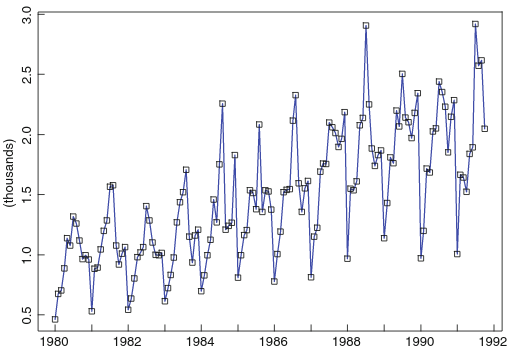
\includegraphics[width=.6\textwidth]{ej-ts}
  \caption{Ejemplo de serie temporal continuo en tiempo discreto. Ventas de vino tinto en Australia 1980-1991.}
  \label{fig:ej-ts}
\end{figure}

\begin{definicion}[Serie temporal]
  Sea un proceso estocástico $\{X_t\}_{t \in T}$, con $X_t : (\Omega, \mathcal{A}, P) \to (E, \mathcal{B}_E), \, \forall t \in T$. Una serie temporal es una realización del proceso estocástico $\{x_t : x_t \in E, t \in T \}$
  \label{def:serie-temporal}
\end{definicion}

Tenemos en cuenta que al hacer una realización obtendremos siempre una cantidad de puntos finitos, que no es excluyente con el hecho de que venga de un proceso en tiempo continuo mientras se haga un muestreo correcto. Además, sea el proceso en tiempo discreto o continuo, generalmente se considera que los tiempos en los que se obtiene la muestra están separados uniformemente.

\subsection{Momentos}

El estudio de los procesos y de las series está profundamente ligado a la predicción de valores: si conseguimos modelar y captar la estructura del proceso podremos predecir valores para tiempos en el futuro. Sin embargo, en general necesitaremos conocer las distribuciones $n$-dimensionales del proceso dadas por la distribución de probabilidad conjunta \eqref{eq:distri-multidim}

\begin{equation}
  P[X_{t_1} \leq x_{t_1}, \ldots, X_{t_n} \leq x_{t_n}], \; \forall \{t_i\}^n_{i = 1} \subseteq T, \; \forall n \in \N.
  \label{eq:distri-multidim}
\end{equation}

Esto en la práctica es muy complicado y poco fáctible de obtener, ya que usualmente solo se tiene una única serie temporal del proceso. Una manera más fácil y útil de describir un proceso es mediante los \textbf{momentos}, en particular los momentos de primer y segundo orden que son las funciones \textbf{media} (\autoref{def:func-media}) y \textbf{autocovarianza} (\autoref{def:func-autocovarianza}) respectivamente.

\begin{definicion}[Función media]
  Sea un proceso estocástico $\{X_t\}_{t \in T}$ que cumple que $E[X_t] < +\infty, \, \forall t \in T$. La función media del proceso se define como:

  $$\begin{aligned} \mu : T & \to \R \\
    t & \mapsto \mu(t) = E[X_t]
  \end{aligned}.$$
  \label{def:func-media}
\end{definicion}

\begin{definicion}[Función autocovarianza]
  Sea un proceso estocástico $\{X_t\}_{t \in T}$ que cumple que $Var[X_t] < +\infty, \, \forall t \in T$. La función media del proceso se define como:

  $$\begin{aligned} \gamma : T \times T & \to \R \\
    (t_1, t_2) & \mapsto \gamma(t_1, t_2) = E\left[(X_{t_1} - \mu(t_1))(X_{t_2} - \mu(t_2))\right] = Cov(X_{t_1}, X_{t_2})
  \end{aligned}.$$
  \label{def:func-autocovarianza}
\end{definicion}

Podemos definir la función \textbf{varianza} como un caso especial de la función autocovarianza cuando $t_1 = t_2$, es decir $\sigma^2(t) = \gamma(t_1, t_1) = Var[X_t]$.

\subsection{Procesos estacionarios}

Una propiedad muy interesante y que puede ayudarnos al modelar los procesos, es la característica de la \textbf{estacionalidad}. De manera informal, un proceso es estacionario si sus propiedades estadísticas (momentos) no cambian con el tiempo.

Veamos que significa formalmente que un proceso sea \textbf{estrictamente estacionario} (\autoref{def:estrictamente-estacionario}).

\begin{definicion}[Proceso estrictamente estacionario]
  Un proceso estocástico $\{X_t\}_{t \in T}$ se dice que es estrictamente estacionario si $\forall n \in N$, $\forall t_1 < \ldots < t_n \in T$, $\forall \tau \in T$ se cumple que:

    $$\left( X_{t_1}, \ldots, X_{t_n}\right) \sim \left( X_{(t_1 + \tau)}, \ldots, X_{(t_n + \tau)}\right).$$
  \label{def:estrictamente-estacionario}
\end{definicion}

Lo que nos dice esta propiedad es que la probabilidad conjunta no cambia si se desplaza, por lo que solo dependerá de la probabilidad conjunta para $t_1, \ldots, t_n$, $\forall n \in N$. De hecho si $n=1$ tendremos que los momentos, si existen, serán todos iguales \eqref{eq:estricto-momentos}

\begin{gather}
  \mu(t) = \mu, \\
  \sigma^2(t) = \sigma^2.
  \label{eq:estricto-momentos}
\end{gather}

Además, si $n = 2$ entonces la distribución conjunta de $X_{t_1}$ y $X_{t_2}$ dependerá solo de la diferencia temporal $(t_2 - t_1) = \tau$ denominada como \textbf{desfase} (\emph{lag}). Por tanto la función autocovarianza puede ser reescrita en función únicamente del desfase, denominándose como \textbf{coeficiente de autocovarianza} con desfase $\tau$ \eqref{eq:estricto-autocovarianza}

\begin{equation}
  \gamma(t_1, t_2) = Cov(X_{t_1}, X_{t_2}) = Cov(X_{0}, X_{(t_2 - t_1)}) = \gamma(0, \tau) = \gamma(\tau).
  \label{eq:estricto-autocovarianza}
\end{equation}

Como las dimensiones del coeficiente de autocovarianza depende de las unidades de medida de $X_t$, por motivos de interpretabilidad se suele estandarizar obteniendo así la función de \textbf{autocorrelación} (ACF) que mide la correlación entre $X_t$ y $X_{t + \tau}$ \eqref{eq:autocorrelacion}

\begin{equation}
  \rho(\tau) = \dfrac{\gamma(\tau)}{\gamma(0)}.
  \label{eq:autocorrelacion}
\end{equation}

Aunque pareciera que no existen muchos procesos que mantengan la misma distribución en todo el tiempo, si existen muchos procesos con una distribución \textbf{de equilibrio}. Estos procesos cumplen que la distribución de probabilidad de $X_t$ tiende a una distribución limite (de equilibrio) cuando $t \to \infty$ y no dependen de las condiciones iniciales. Por tanto si las condiciones iniciales se fijan para ser iguales que la distribución de equilibrio, el proceso es fuertemente estacionario.

Sin embargo, podemos relajar las condiciones de la estacionalidad para hacerlas más prácticas en casos reales, poniendo únicamente condiciones a los momentos de primer y segundo orden. Definimos los procesos \textbf{débilmente estacionarios} o \textbf{estacionarios de segundo orden} como \autoref{def:debilmente-estacionario}

\begin{definicion}[Proceso débilmente estacionario]
  Sea un proceso estocástico $\{X_t\}_{t \in T}$, se dice que el proceso es débilmente estacionario o estacionario de segundo orden si se cumple lo siguiente:

  \begin{enumerate}
    \item $\mu(t) = \mu, \, \forall t \in T$.
    \item $\gamma(t_1, t_2) = \gamma  (t_1 + \tau, t_2 + \tau), \, \forall t_1, t_2, \tau \in T$
  \end{enumerate}

  La condición 2, como ya vimos, implica que $\gamma(t_1, t_2) = \gamma(\tau)$.
  \label{def:debilmente-estacionario}
\end{definicion}

Obviamente que un proceso sea fuertemente estacionario implica que sea débilmente estacionario pero no al revés. De hecho la doble implicación se da si el proceso tiene una distribución conjunta normal multivariante, ya que en ese caso queda determinada por los momentos de primer y segundo orden.

El \textbf{ruido independiente idénticamente distribuido} (ruido iid.) es el ejemplo básico de proceso estrictamente estacionario (\autoref{def:ruido-iid}).

\begin{definicion}[Ruido iid]
  Un proceso $\{X_t\}_{t \in T}$ estocástico se dice que es ruido independiente idénticamente distribuido con media $\mu$ y varianza $\sigma^2$, denotado por $\{X_t\} \sim IID(\mu, \sigma^2)$, si todas las variables aleatorias $X_t$ son independientes e idénticamente distribuidas con $E[X_t] = \mu, Var[X_t] = \sigma^2, \, \forall t \in T$.
\label{def:ruido-iid}
\end{definicion}

Debido a la independencia de las variables tendremos que la función media del proceso será $\mu$, y la función autocovarianza será \eqref{eq:autocov-ruido}

\begin{equation}
  \gamma(\tau) =
  \begin{cases}
    \sigma^2, & \tau = 0 \\
    0, & \tau \neq 0
  \end{cases},
  \label{eq:autocov-ruido}
\end{equation}

que no depende del tiempo $t$ y junto a la independencia de las variables nos dice que el proceso es estrictamente estacionario.

Uno puede relajar la condición de independencia e distribución idéntica para obtener un tipo de proceso débilmente estacionario, el llamado \textbf{ruido blanco} (\autoref{def:ruido-blanco}).

\begin{definicion}[Ruido blanco]
  Un proceso $\{X_t\}_{t \in T}$ estocástico se dice que es ruido blanco (\emph{white noise}) con media $\mu$ y varianza $\sigma^2$, denotado por $\{X_t\} \sim WN(\mu, \sigma^2)$, si todas las variables aleatorias $X_t$ son incorreladas con $E[X_t] = \mu, Var[X_t] = \sigma^2, \, \forall t \in T$.
\label{def:ruido-blanco}
\end{definicion}

En este caso el ruido blanco obtiene la misma función media y autocovarianza que el ruido iid. \eqref{eq:autocov-ruido} haciendo que el proceso sea débilmente estacionario. Así, cualquier proceso $IID(\mu, \sigma^2)$ es $WN(\mu, \sigma^2)$ pero no al revés.

Para ambos procesos podemos calcular la función de autocorrelación \eqref{eq:ruido-autocorrelacion}

\begin{equation}
  \rho(\tau) =
  \begin{cases}
    1, & \tau = 0 \\
    0, & \tau \neq 0
  \end{cases}.
  \label{eq:ruido-autocorrelacion}
\end{equation}

Mostramos un ejemplo de un proceso $\{X_n\}_{n = 1}^{500} \sim IID(0, 1)$ generado con $X_n \sim N(0, 1), \, n = 1, \ldots, 500$ junto con su correlograma (el valor de la función de autocorrelación en función del desfase) (\autoref{fig:ruido-ej}, \cite{chatfield2019analysis}).

\begin{figure}[htpb]
  \centering
  %\hspace*{-2.5cm}
  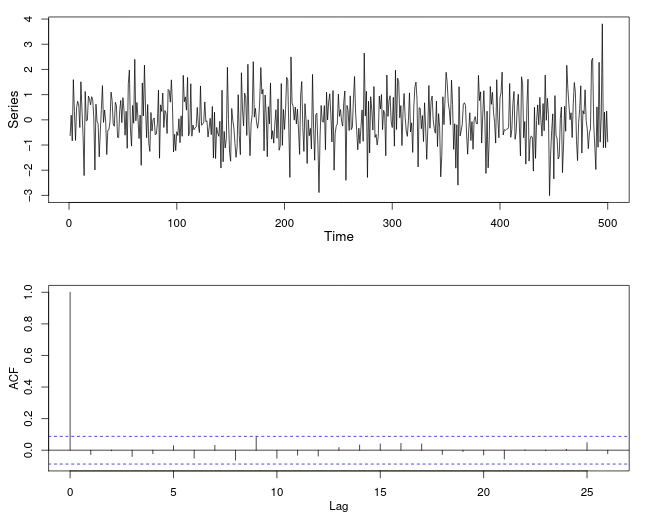
\includegraphics[width=.8\textwidth]{ruido-iid}
  \caption{Proceso $IID(0, 1)$ con su correlograma.}
  \label{fig:ruido-ej}
\end{figure}

Un proceso muy simple que no es estacionario es el \textbf{camino aleatorio} (\autoref{def:random-walk})

\begin{definicion}[Camino aleatorio]
  Se dice que un proceso $\{X_t\}_{t \in T}$ es un camino aleatorio si

  $$X_t = X_{t - 1} + Z_t, \, \forall t \in T,$$

  donde $\{Z_t\}_{t \in T} \sim IID(\mu , \sigma^2)$. Generalmente cuando $t = 1$ se toma $X_1 = Z_1$, haciendo que el proceso sea como:

  $$X_t = \sum \limits^t_{i = 1} Z_i, \, \forall t \in T.$$
  \label{def:random-walk}
\end{definicion}

Para un camino aleatorio se tiene debido a la independencia de $Z_t$ que $E[X_t] = t \mu$ y $Var[X_t] = t \sigma^2$. Como dependen de $t$ el proceso no es estacionario.

Podemos generar caminos aleatorios fácilmente mediante un proceso $IDD(\mu, \sigma^2)$ (\autoref{fig:ej-random-walk}, \cite{chatfield2019analysis}).

\begin{figure}[htpb]
  \centering
  %\hspace*{-2.5cm}
  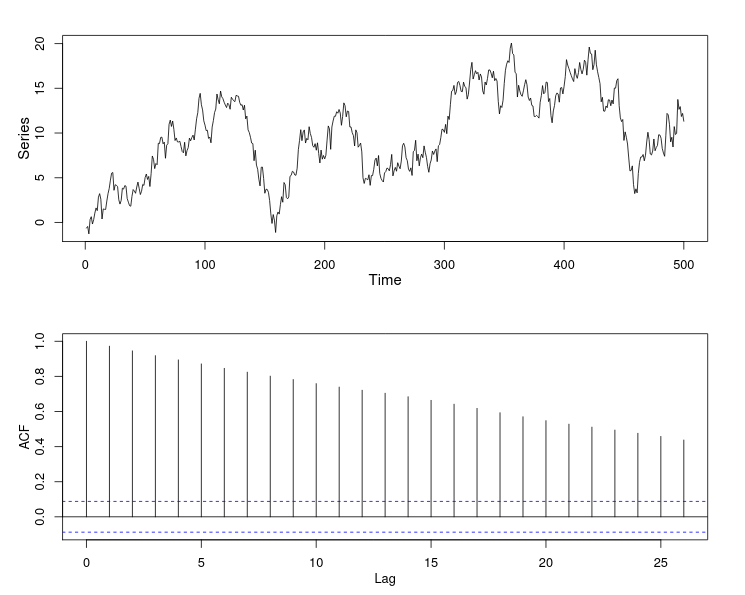
\includegraphics[width=.8\textwidth]{random-walk-ej}
  \caption{Ejemplo de camino aleatorio generado con ruido, junto con su correlograma.}
  \label{fig:ej-random-walk}
\end{figure}

\section{Descomposición}

Una parte importante del análisis de series se centra en el modelado de los procesos mediante la descomposición en varias componentes que suelen exhibir. Veremos cuáles son estas componentes y distintas maneras para obtener esta descomposición.

\subsection{Patrones}

Listemos los patrones fundamentales que muestran muchas series:

\begin{itemize}
  \item \textbf{Tendencia}: un cambio a largo plazo en el nivel medio de la serie, que puede ser creciente o decreciente.
  \item \textbf{Variación estacional}: un patrón que se repite cada cierto periodo de tiempo fijo debido a factores estacionales (cada estación, o año).
  \item \textbf{Variaciones cíclicas}: fluctuaciones de las series sin frecuencia fija y que pueden cambiar a lo largo del tiempo.
\end{itemize}

Veamos ejemplos de estos patrones en \autoref{fig:patrones-ej} \cite{hyndman2018forecasting}.

\begin{figure}[htpb]
  \centering
  %\hspace*{-2.5cm}
  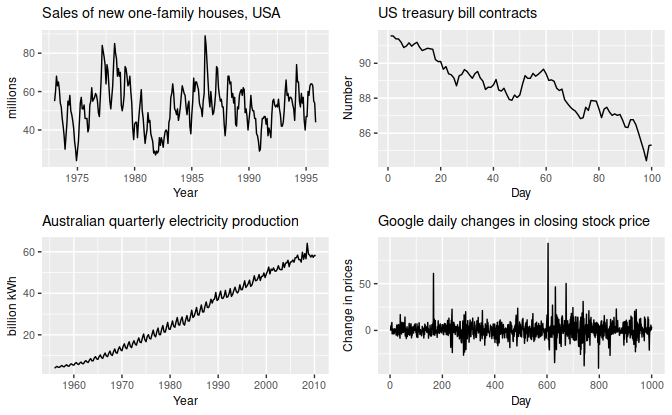
\includegraphics[width=.9\textwidth]{patrones-ejemplos}
  \caption{Ejemplos de series con distintos patrones.}
  \label{fig:patrones-ej}
\end{figure}

Analicemos cada serie para observar los patrones en cada una:

\begin{itemize}
  \item Arriba-izquierda: se muestra un carácter estacional cada año, junto con patrones cíclicos que van variando.
  \item Arriba-derecha: únicamente tendencia decreciente.
  \item Abajo-izquierda: tendencia creciente junto a una variación estacional de un año.
  \item Abajo-derecha: sin ningún patrón observable, son fluctuaciones aleatorias.
\end{itemize}

En base a estos patrones, el análisis clásico de series temporales se basa en la descomposición de estas en los componentes que hemos comentado \eqref{eq:decomposition}

\begin{equation}
  X_t = m_t + s_t + Y_t, \, \forall t \in T,
  \label{eq:decomposition}
\end{equation}

donde $m_t$ es la componente de la tendencia-ciclos (que se dice solamente tendencia), $s_t$ la componente estacional e $Y_t$ ruido aleatorio (débilmente) estacionario.

Esta descomposición se dice que es \textbf{aditiva} pues suma sus componentes y existe otra forma llamada \textbf{multiplicativa}, que suele ser útil cuando las fluctuaciones de la serie son proporcionales al tiempo de la serie \eqref{eq:decomposition-mult}

\begin{equation}
  X_t = m_t \cdot s_t \cdot Y_t, \, \forall t \in T.
  \label{eq:decomposition-mult}
\end{equation}

El enfoque general consiste en extraer de las series estas componentes $m_t$, $s_t$ y esperar que el ruido $Y_t$ sea estacionario. Usando la teoría que hemos visto, creamos un modelo para el proceso en el que podemos simular valores junto con $m_t$ y $s_t$.

Existe otra técnica que consiste en aplicar operadores para diferenciar la serie hasta que las observaciones se parezcan a una serie estacionaria, volviendo a usar la teoría para modelar los procesos.

\subsection{Descomposición sin estacionalidad}

Si tenemos un proceso que no presenta la componente estacional entonces obtenemos el siguiente modelo (\autoref{def:solo-tendencia})

\begin{definicion}[Descomposición con solo tendencia]
  Sea $\{X_t\}$ un proceso entonces una descomposición con solo tendencia está definida por:

  $$ X_t = m_t + Y_t, \; \forall t \in T,$$

  donde $m_t$ es la tendencia e $Y_t$ los residuos y se tiene que $E[Y_t] = 0, \forall t \in T$. Si esto último no fuese así, el modelo se cambiaría por:

  $$ X_t = (m_t + E[Y_t]) + (Y_t - E[Y_t]), \; \forall t \in T.$$
  \label{def:solo-tendencia}
\end{definicion}

\subsubsection{Ajuste polinómico}

Para poder estimar la tendencia $m_t$ podemos utilizar varias técnicas. La primera de ellas es la más simple y conocida: el \textbf{ajuste polinómico} (\autoref{def:ajuste-polinomico}).

\begin{definicion}[Ajuste polinómico]
  Sea un $\{X_t\}_{t = 1}^n$ un proceso y $\{x_t\}_{t = 1}^n$ una serie temporal observada del proceso. El ajuste polinómico de gradp $k$ considera que la tendencia es un polinomio de grado $k$ de la forma

  $$m_t = \sum \limits^k_{i = 0} a_i t^i,$$

  La tendencia estimada $\hat{m}_t$ determinada por los parámetros $\hat{a}_0, \hat{a}_1, \ldots, \hat{a}_k$ se obtienen al minimizar el error cuadrático medio $$\sum \limits^n_{t = 1} (x_t - m_t)^2.$$
  \label{def:ajuste-polinomico}
\end{definicion}

\autoref{fig:ajuste-ej} (\cite{brockwell2002introduction}) nos muestra un ejemplo de ajuste polinómico de grado 2 (cuadrático) donde se estima $\hat{m}_t = \hat{a}_0 + \hat{a}_1 t + \hat{a}_2 t^2$ a través de la serie observada.

\begin{figure}[htpb]
  \centering
  %\hspace*{-2.5cm}
  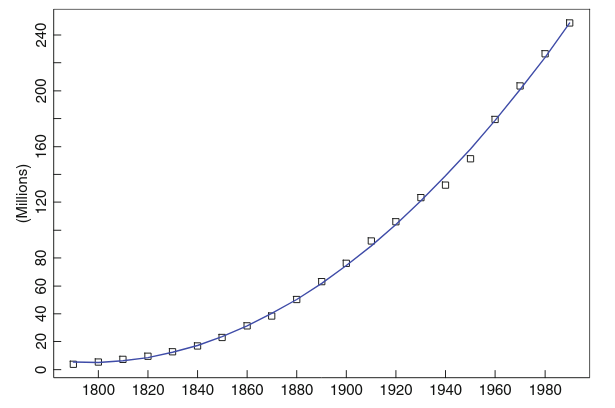
\includegraphics[width=.6\textwidth]{ajuste-ej}
  \caption{Ajuste cuadrático de la población en EE.UU. entre 1790-1990.}
  \label{fig:ajuste-ej}
\end{figure}

\subsubsection{Suavizado con media móvil}

La siguiente técnica consiste en estimar la tendencia mediante el \textbf{suavizado con media móvil} (\autoref{def:suavizacion-media})

\begin{definicion}[Suavizado con media móvil]
  Sea un proceso $\{X_t\}_{t = 1}^n$, y un natural $q \in N$. Se define el proceso suavizado con media móvil simétrica de orden $q$ de $\{X_t\}$ como:

  $$ W_t = \dfrac{1}{2q + 1} \sum \limits^q_{i = -q} X_{t - i}, \, \forall t = 1, \ldots, n.$$
  \label{def:suavizacion-media}
\end{definicion}

Asumiendo que $m_t$ es aproximadamente lineal en el intervalo $[t - q, t + q]$ y que la media de los errores en el mismo intervalo es aproximadamente cero, aplicamos el suavizado al modelo \autoref{def:solo-tendencia} obteniendo \eqref{eq:suavizacion}

\begin{equation}
  W_t = \dfrac{1}{2q + 1} \sum \limits^q_{i = -q} m_{t - i} + \dfrac{1}{2q + 1} \sum \limits^q_{i = -q} Y_{t - i} \approx m_t, \; t = q + 1, \ldots, n - q.
  \label{eq:suavizacion}
\end{equation}

Por tanto la tendencia estimada para un proceso $\{X_t\}_{t = 1}^n$ quedaría como \eqref{eq:suavizacion-estimada}

\begin{equation}
  \hat{m}_t = \dfrac{1}{2q + 1} \sum \limits^q_{i = -q} X_{t - i}, \; t = q + 1, \ldots, n - q.
  \label{eq:suavizacion-estimada}
\end{equation}

Notamos que $\hat{m}_t$ no está definida para $t > n - q$ o $t \leq q$ que podría dejarse así o extender los términos definiendo $X_t := X_1, \forall t < 1$ y $X_t := X_n, \forall t > n$.

Un ejemplo de $\hat{m}_t$ aplicando un suavizado de media móvil con $q = 2$ (5 términos) lo tenemos en \autoref{fig:ej-suavizacion} (\cite{brockwell2002introduction}).

\begin{figure}[htpb]
  \centering
  %\hspace*{-2.5cm}
  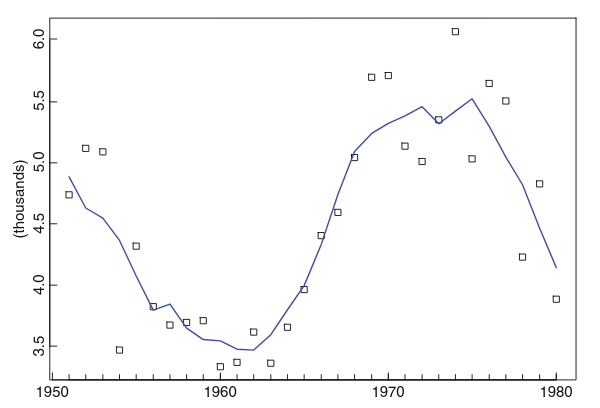
\includegraphics[width=.6\textwidth]{ej-suavizacion}
  \caption{Suavizado con media móvil con 5 términos del número de huelgas en EE.UU entre 1951-1980.}
  \label{fig:ej-suavizacion}
\end{figure}

\subsubsection{Suavizado exponencial}

Finalmente consideramos una técnica que realiza el suavizado como una combinación entre el punto $t$-ésimo actual y el punto estimador anterior (\autoref{def:suavizado-exponencial})

\begin{definicion}[Suavizado exponencial]
  Sea $\{X_t\}_{t = 1}^n$ un proceso y $\alpha \in [0, 1]$, el suavizado exponencial se define como la estimación de la tendencia del proceso de la siguiente forma:

  $$\hat{m}_t = \alpha X_t + (1 - \alpha)\hat{m}_{t - 1}, \; t = 2, \ldots, n,$$

  donde $\hat{m}_1 = X_1$.
  \label{def:suavizado-exponencial}
\end{definicion}

Este método se denomina suavizado exponencial debido a que $\forall t \geq 2$ se cumple \eqref{eq:exponencial-desarrollada}

\begin{equation}
  \hat{m}_t = \sum \limits^{t - 2}_{i = 1} \alpha(1 - \alpha)^i X_{t - i} + (1 - \alpha)^{t - 1} X_1,
  \label{eq:exponencial-desarrollada}
\end{equation}

donde se puede ver el proceso estimado como una media móvil con pesos decrecientes exponencialmente. Un ejemplo lo tenemos en \autoref{fig:ej-suavizado} (\cite{brockwell2002introduction})

\begin{figure}[htpb]
  \centering
  %\hspace*{-2.5cm}
  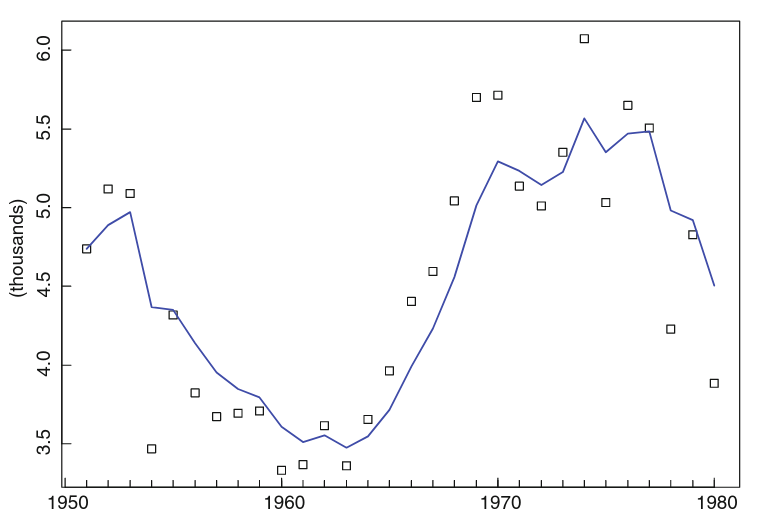
\includegraphics[width=.6\textwidth]{ej-suavizado}
  \caption{Suavizado exponencial con $\alpha = 0.6$ en el número de huelgas.}
  \label{fig:ej-suavizado}
\end{figure}

\subsection{Descomposición completa}

Ahora consideramos la descomposición completa, añadiendo al modelo que hemos estado utilizando la componente estacional. Esperamos que esta componente se repita siempre cada cierto periodo de tiempo $T$ y además que la suma de los valores en un periodo sea cero (\autoref{def:descomposicion-entera}).

\begin{definicion}[Descomposición completa]
  Sea $\{X_t\}$ un proceso entonces una descomposición completa está definida por:

  $$ X_t = m_t + s_t + Y_t, \; \forall t \in T,$$

  donde $m_t$ es la tendencia, $s_t$ es la estacionalidad con periodo $T$ e $Y_t$ los residuos.  Además se tiene que $E[Y_t] = 0$, $s_{t + T} = s_{t}$ y $\sum \limits^{T}_{i = 1} s_i = 0$, $\forall t \in T$.
  \label{def:descomposicion-entera}
\end{definicion}

\subsubsection{Descomposición clásica}

Explicaremos el método clásico básico para obtener una descomposición de un proceso ya que es el funcionamiento básico del resto de descomposiciones que han ido surgiendo.

El primer paso es estimar la tendencia $\hat{m}_t$ mediante una media móvil con pesos especiales para eliminar la estacionalidad y disminuir el ruido. Si el periodo $T$ es par, elegimos $q = T / 2$ y obtenemos la estimación como \eqref{eq:decomp-1}

\begin{equation}
  \hat{m}_t = \dfrac{\dfrac{1}{2}X_{t - q} + X_{t-q+1} + \cdots + X_{t+q+1} + \dfrac{1}{2}X_{t + q}}{T}, \; t = q + 1, \ldots, n - q,
  \label{eq:decomp-1}
\end{equation}

y si el periodo es impar tomamos $q = (d-1)/2$ y estimando como \eqref{eq:decomp-2}

\begin{equation}
  \hat{m}_t = \dfrac{X_{t - q} + X_{t-q+1} + \cdots + X_{t+q+1} + X_{t + q}}{T}, \; t = q + 1, \ldots, n - q.
  \label{eq:decomp-2}
\end{equation}

El siguiente paso es estimar la componente estacional $\hat{s}_t$, para ello primero calculamos la media de las desviaciones de la serie respecto la tendencia estimada \eqref{eq:decomp-3}

\begin{equation}
  w_t = \dfrac{T}{n - 2q} \sum \limits^{\frac{n - q - t}{T}}_{i = \frac{q - t}{T} + 1} \left(X_{t + iT} - \hat{m}_{t + iT}\right), \; t = 1, \ldots, T,
  \label{eq:decomp-3}
\end{equation}

que ajustamos para conseguir que la suma sea 0 \eqref{eq:decomp-4}

\begin{equation}
  \hat{s}_t = w_t - \dfrac{1}{T}\sum \limits^T_{i = 1} w_i, \; t = 1, \ldots, T.
  \label{eq:decomp-4}
\end{equation}

Es posible obtener la serie sin la componente sin estacionalidad \eqref{eq:decomp-5}

\begin{equation}
  d_t = X_t - \hat{s}_t, \; t = 1, \ldots, n,
  \label{eq:decomp-5}
\end{equation}

de manera que ahora podemos descomponer $\{d_t\}_{t = 1}^n$ para obtener solamente la tendencia usando un ajuste polinómico. Este paso es posible no realizarlo, pero es interesante tener una forma paramétrica para la tendencia que puede ser extrapolada fácilmente.

Finalmente obtenemos estimamos la componente de residuos \eqref{eq:decomp-6}

\begin{equation}
  \hat{Y}_t = X_t - \hat{m}_t - \hat{s}_t, \; t = 1, \ldots, n.
  \label{eq:decomp-6}
\end{equation}

Un ejemplo de descomposición de un proceso lo tenemos en \autoref{fig:ej-descomposicion} (\cite{hyndman2018forecasting}).

\begin{figure}[htpb]
  \centering
  %\hspace*{-2.5cm}
  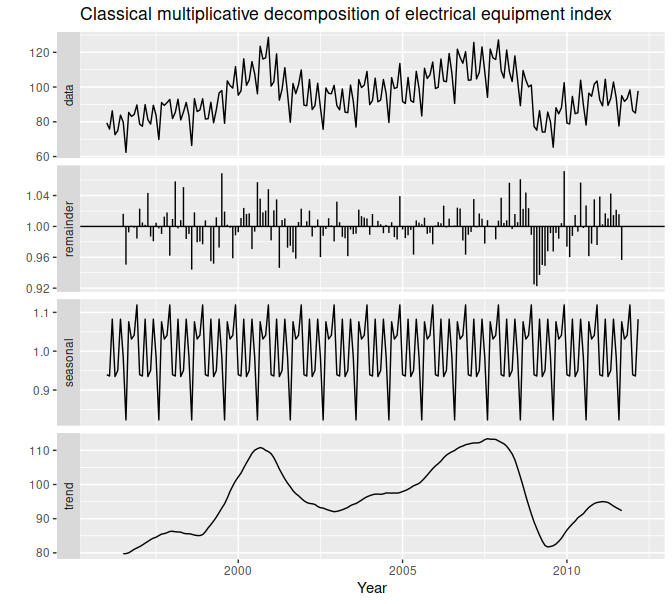
\includegraphics[width=.65\textwidth]{ej-descomposicion}
  \caption{Ejemplo de descomposición clásica de una serie.}
  \label{fig:ej-descomposicion}
\end{figure}

\subsubsection{Otras descomposiciones}

Existen otras descomposiciones que modifican el método que hemos descrito, entre ellas destacan la descomposición X11 \cite{shiskin1965x, dagum2016seasonal} o SEATS (\emph{Seasonal Extraction in ARIMA Time Series}) \cite{gomez1995programs, dagum2016seasonal}.

Una de las descomposiciones más famosas y la que usaremos en el proyecto será la descomposición STL (\emph{Sesonal and Trend decomposition using Loess}) \cite{cleveland1990stl}. Mostramos como ejemplo la descomposición de la serie que habíamos utilizado para la descomposición clásica \autoref{fig:stl-decomposition} (\cite{hyndman2018forecasting}).

\begin{figure}[htpb]
  \centering
  %\hspace*{-2.5cm}
  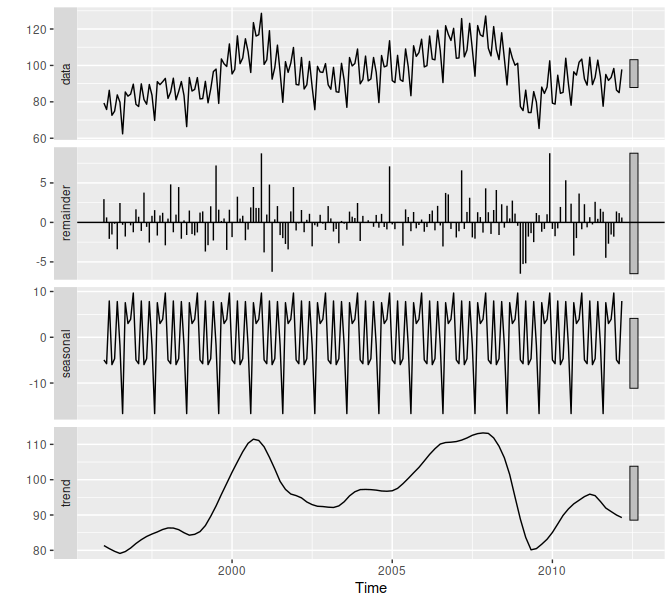
\includegraphics[width=.65\textwidth]{stl-decomposition}
  \caption{Ejemplo de descomposición STL de una serie.}
  \label{fig:stl-decomposition}
\end{figure}

\endinput
